 \documentclass [12pt]{article}
\usepackage{geometry}
 \geometry{
 a4paper,
 left=25mm,
 right=25mm,
 top=30mm,
 bottom=30mm,
 headsep=10mm,
 footskip=15mm}
\linespread{1.175}\selectfont
\usepackage{blindtext}
\usepackage[utf8]{inputenc}
\usepackage[english]{babel}
\def\labelitemi{--}
\def\labelitemii{*}
\pagenumbering{arabic}
\usepackage[hidelinks]{hyperref}
\usepackage{fancyhdr}
\usepackage[shortlabels]{enumitem}
\usepackage{wrapfig}
\pagestyle{fancy}
\fancyhf{}
\lhead{\small{Travlendar+ project by Meneghin Giulia \& Mauri Giuseppe}}
\rhead{\small{\rightmark}}
\rfoot{\small{Page \thepage}}
\lfoot{\small{Copyright © 2017, Meneghin Giulia \& Mauri Giuseppe  – All rights reserved}}

\setlength{\headheight}{17pt}
\usepackage{graphicx}
\newcommand{\sectionbreak}{\clearpage}
\usepackage{titlesec}
\usepackage{hyperref}
\usepackage{subcaption}
\usepackage{tabu}
\begin{document}

\begin{figure}[ht!]
\centering

\includegraphics[height=5.8cm,width=5.8cm]{logopoli.png}
\end{figure}
\begin{large}
\centerline{\textbf{Politecnico di Milano} }
\centerline{AA 2017-2018}
\vspace{0.5cm}
\centerline{Computer Science and Engineering}
\centerline{\textbf{Software Engineering 2 Project}}
\end{large}
\begin{figure}[ht!]
\centering

\includegraphics[width=\linewidth]{Immaginecopertina.png}
\end{figure} 

\clearpage

\begin{table}[h!]
\begin{tabu} to \textwidth { X[0.3,r,p] X[0.7,l,p] }
\hline

\textbf{Deliverable:} & DD\\
\textbf{Title:} & Design Document \\
\textbf{Authors:} & Meneghin Giulia \& Mauri Giuseppe \\
\textbf{Version:} & 1.0 \\ 
\textbf{Date:} & 26-November-2017 \\
\textbf{Download page:} & \url{<https://github.com/Ciuse/MauriMeneghin>} \\
\textbf{Copyright:} & Copyright © 2017, Meneghin Giulia \& Mauri Giuseppe – All rights reserved \\
\hline
\end{tabu}
\end{table}

\clearpage

\tableofcontents

\section{Introduction}
\subsection{Purpose}
\subsection{Goals}
\begin{enumerate}
\item[(G1)]Allow the user of the application to create a personal account and modify his information.


\end{enumerate}
\subsection{Functional Requirement}
\begin{description}

\item[(G1)]Allow the user of the application to create a personal account and modify his information.
\end{description}
\begin{itemize}
\item The user should be able to register through the mobile application.\\
The user must provide user-name, password, e-mail, and a valid address that will be used as the default position.\\
\item The user must insert the transport means preferences.\\
Then he can accept or modify the default limits about them.\\
\item Finally, he can accept or modify the default set of “Type of appointment”.\\
\item The user must be able to modify all the option even after he finished the registration process.\\
\end{itemize}
\subsection{Scope}

\subsection{Acronyms}
\begin{itemize}
\item\textit{API:} Application Programming Interface.
\end{itemize}

\subsection{Revision history}
\begin{itemize}
\item Version 1.0
\end{itemize}

\subsection{Document Structure}


\subsubsection{Introduction:}
The introduction to this section describes the main features of the design document. This section highlights more technical aspects that were not dealt with in the RASD document. We can distinguish different subsections of this document:
\subsubsection{Architecture Design:}
\begin{itemize}
\item Overview: The top-level components of our application are described.
\item High level components and their interaction: This section focuses on how the various components interact with each other.
\item Component View: This section provides a more detailed view of the application components. We will use the component diagram which will show how the components of our application are connected together to form larger components. The system structure is shown.
\item Deployment View: This section shows how software components are distributed over the hardware resources available on your system. We will use a Deployment Diagram that statically describes our system in terms of hardware resources, called nodes, and relationships between them.  
\item Runtime view: In this part, sequence diagrams will be used to describe how components interact to perform specific tasks typically related to usage cases.
\item Component interfaces
\item Selected architectural styles and models: This section explains the architectural choices made during the implementation of the application.
\item Other design decisions
\end{itemize}
\subsubsection{System interfaces}

\subsubsection{Software interfaces}

\subsubsection{Algorithms Design:}

\subsubsection{User Interface Design:}
This section presents examples of mockups and user experiences.
\subsubsection{Requirements Traceability:}
This section explains how decisions taken in the RASD are related to design elements.
\subsubsection{Implementation, Integration and Test Plan:}
This last section proposes the order in which we plan to implement the sub-components of our system and the order in which we plan to integrate these sub-components and test the integration.
\section{Architectural Design}
\subsection{Overview}

\subsection{High level components}


\subsection{Component view}

\null
\vspace{\stretch{2}}
\begin{figure}[ht!]
\centering
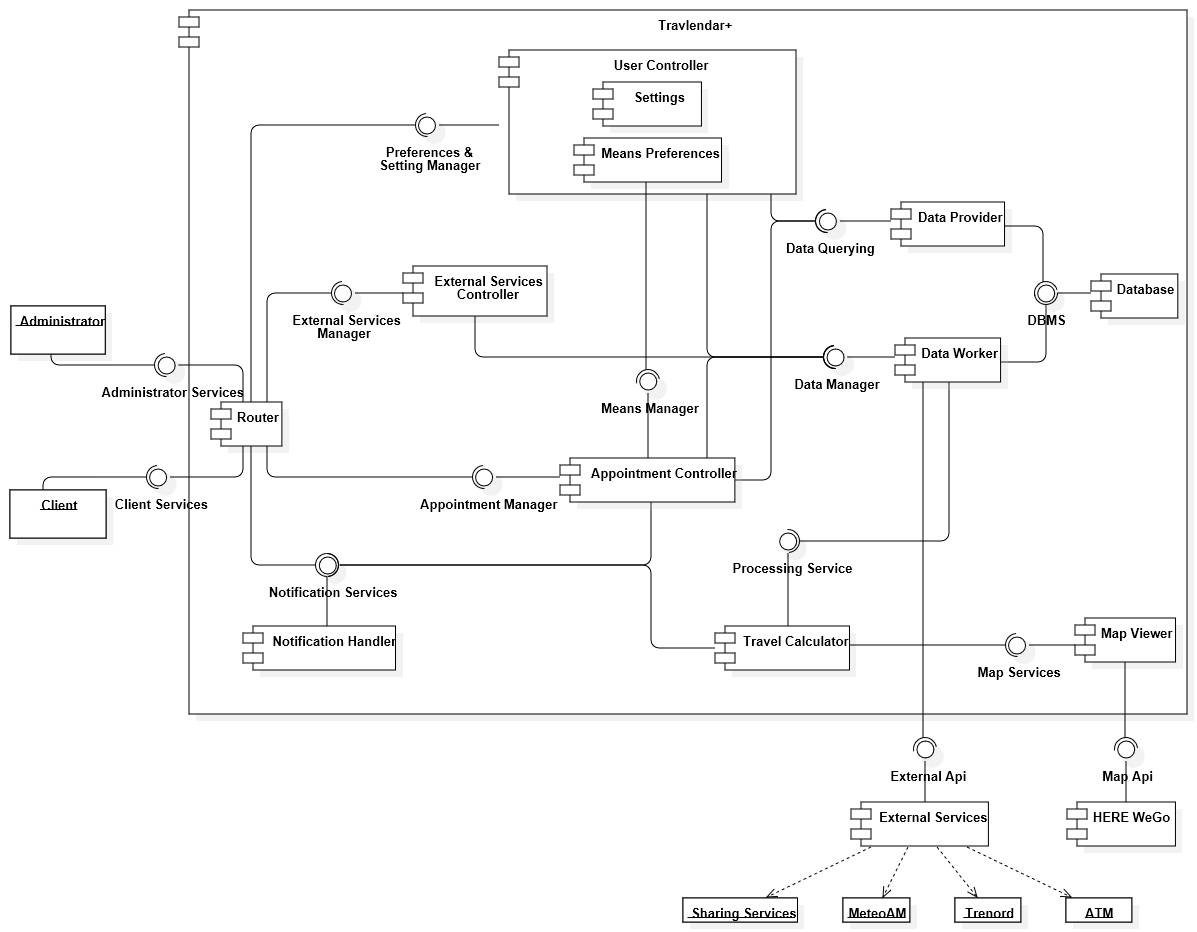
\includegraphics[height=14cm, width=\linewidth]{ComponentDiagram1.jpg}
\caption{Component Diagram}
\end{figure}  
\vspace{\stretch{5}}
\clearpage


\begin{itemize}[•]
\item Client:  the client’s device (mobile app).
\item Administrator: the administrator’s device (mobile app).
\end{itemize}
\clearpage

\subsection{Runtime view}
In the following Sequence Diagram for simplicity and clarity, some steps have been omitted in the communication between the components external to the main system and the router; as the main aspects of communication, between the User and the Travlendar system, have been dealt with in the RASD document.

\null
\vspace{\stretch{2}}
\subsubsection{Sequence Diagram 1}
This Sequence Diagram deals with the addition of an appointment by the customer. The request is taken on board by the router, which communicates with the appointments component and will show the user the form to fill in the data concerning his new event.\\
Subsequently, after the user has inserted the various information, the Appointment Controller component will check that it does not overlap with an existing one, in case the Notification Manager will send the user an error.\\
If the appointment is valid, the data worker will be asked to save the new appointment on the database and the latter will be responsible for providing the travel calculator with all the data necessary to calculate the trip from the previous position to that of the appointment, with the means and preferences that the user has selected.\\
If it is possible to solve the calculation, the travel itinerary will be saved and the user will receive a confirmation message; if not, it will be notified with a warning.
\vspace{\stretch{5}}
\\

\begin{figure}[ht!]
\centering
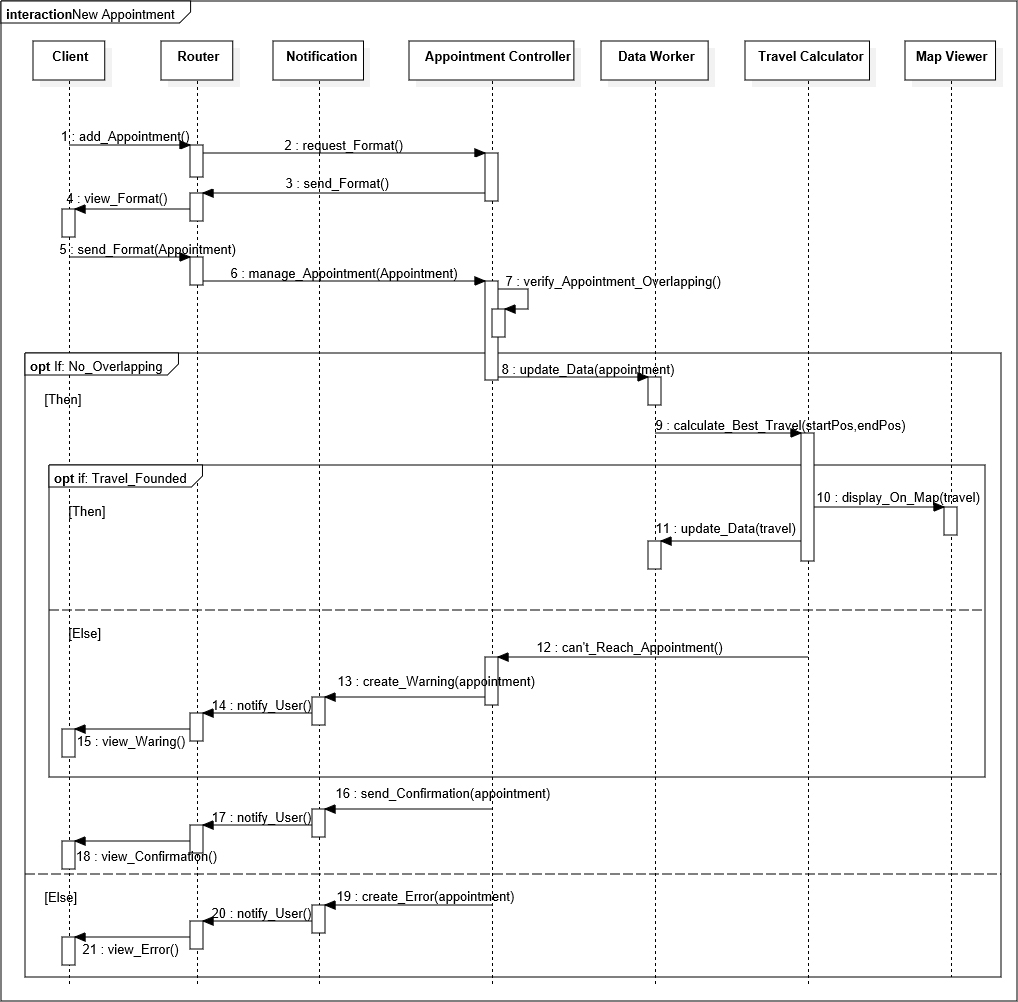
\includegraphics[height=19cm, width=\linewidth]{SQ1.jpg}
\caption{Sequence Diagram 1}
\end{figure}  
\clearpage

\subsection{Component interfaces}

\subsubsection{Administrator Services}
\begin{figure}[ht!]
\centering
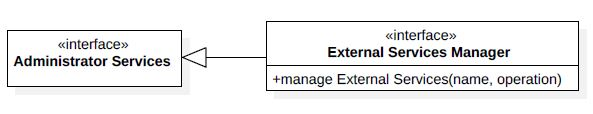
\includegraphics[height=3cm, width=12.5cm]{Int1.jpg}
\end{figure}
\subsubsection{Client Services}
\begin{figure}[ht!]
\centering
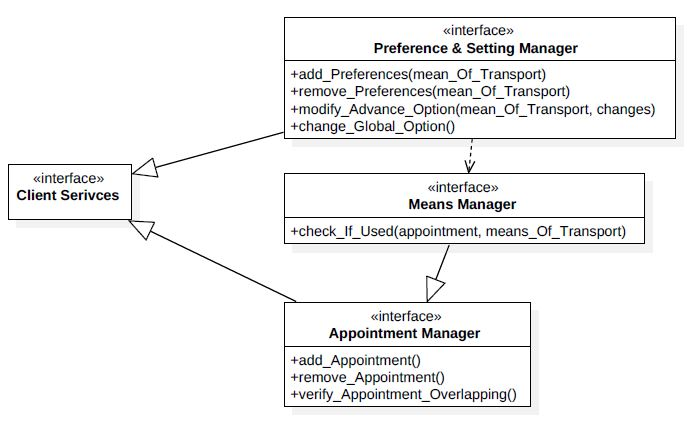
\includegraphics[height=7.5cm, width=14.5cm]{Int2.jpg}
\end{figure}
\subsubsection{DBMS}
\begin{figure}[ht!]
\centering
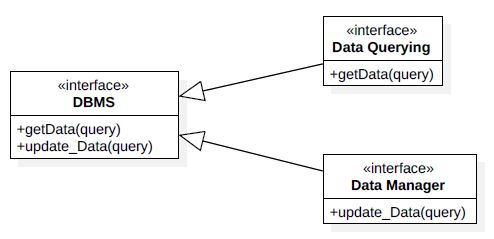
\includegraphics[height=5cm, width=12cm]{Int3.jpg}
\end{figure}
\clearpage
\subsubsection{Processing Service}
\begin{figure}[ht!]
\centering
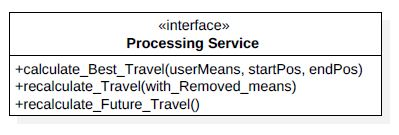
\includegraphics[height=3.3cm, width=8cm]{Int4.jpg}
\end{figure}
\subsubsection{Notification Service}
\begin{figure}[ht!]
\centering
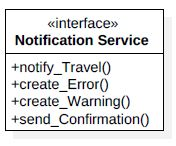
\includegraphics[height=3.3cm, width=4.8cm]{Int5.jpg}
\end{figure}
\subsubsection{Map Service}
\begin{figure}[ht!]
\centering
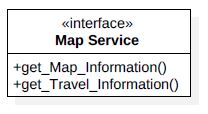
\includegraphics[height=3.0cm, width=5.5cm]{Int6.jpg}
\end{figure}
\subsubsection{API Interface}
\begin{figure}[ht!]
\centering
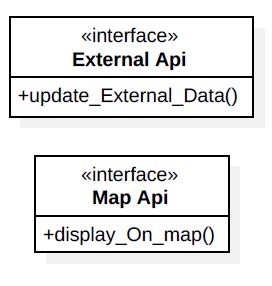
\includegraphics[height=5cm, width=5cm]{Int7.jpg}
\end{figure}


\subsection{Styles and patterns}
\subsubsection{Overall Architecture}

\begin{figure}[ht!]
\centering
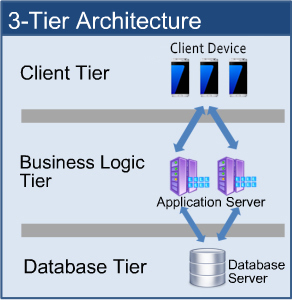
\includegraphics[height=7cm, width=7cm]{3tier.jpg}
\end{figure}  
Our application will be divided into 2 tiers: (fat client)
\begin{enumerate}
\item Database tier ( DAL: Data Access Layer )
\item Business Logic tier ( BLL: Business Logic Layer ) (mobx)
\item Client tier (interface to BLL )
\end{enumerate}


\subsubsection{Design decisions}

\subsubsection{Design patterns}

\section{Algorithm design}

\subsection{Brief description of the best travel calculation algorithm}

\subsection{Software System Attributes} 

\subsubsection{Reliability}
The users age range is 16-40 years old, so the system will be designed to be always reliable:
\begin{itemize}
\item On workday, in the early morning (7-10) and in the late afternoon (16-19); 
\item On weekend, from the midday to middle evening (11-16) and in the evening (19-24);
\end{itemize}
Because during the working day the user will use the application mainly for register his working or studying appointment and some personal engagements.\\
While in the weekend the user will register his leisure events and night friends meeting.

\subsubsection{Availability}
The system must guarantee a 24/7 service. Very small interrupt of the service during the day will be acceptable and tolerated. But when an issue occurs, the system must respond correctly after a maximum of 3 user attempts.
\subsubsection{Security}
Users credentials and external services account will be cryptate and stored in a reserved and protect area of the system database. Also, the privacy information about the user movement and his localization must be all encrypted and totally protected.
\subsubsection{Maintainability}
Our system uses many external APIs, so the maintainability of our software is very much dependent on this factor. Our system must always be updated with external API interfaces, and it must always be able to interpret and exploit the data it obtains from them.
Generally, there should not be too much invasive maintenance processes, as it uses very popular APIs used by many other software, whose changes are often minimal and well documented.
\subsubsection{Portability}
The system in terms of portability shall be very flexible. The application logic and the system interfaces are abstractly separated; so, the application porting consist only in the re-adapting of the user interface with the new operating system.
Also, could be necessary to reimplement some of the system interaction with the external services.\\

\section{User Interface Design}


\section{Implementation,Integration and Test Plan:}
\subsection{Elements to be integrated}

\subsection{Integration Testing Strategy}

\subsection{Component Integration}

\subsection{Used Tools}
\begin{itemize}
\item StarUml 2.8.0
\item Miktex 2.9.6361
\item Texmaker 5.0.2
\item DeepL
\item GitHubDesktop 1.0.6
\item AdobePhotoshop CC 2017
\item Power Point
\end{itemize}
\end{document}